\chapter{Lec 07 - Neural Networks I}

\section{Introduction}
There are a lot of different neural networks models which answer different computational/learning needs:
\begin{itemize}
    \item \textbf{Supervised learning} (classification, regression, time series prediction, ...)
    
    \item \textbf{Unsupervised learning} (clustering, representation learning, ...)

\end{itemize}
All these models differ for: Network topology, function computed by single neurons, training algorithm and how the training proceeds.\newline\newline
Characteristics of the problem:
\begin{itemize}
    \item Input: discrete and/or real-valued vectors.
    \item Output: discrete (classification) or real-valued (regression) vectors.
    \item Data (input and/or output) can be noisy (e.g. the same instance has two different labels) and the form of the target function is unknown. Note that having no assumption on the target function is not always a pro, but can be a problem.
    \item Having long learning time is acceptable and a quick evaluation of the learned function is required. These models can be used, for example, for real time predictions.
    \item The final solution does not need to be understood by a human expert ("\textit{black box problem}").
\end{itemize}
Examples of application of Neural Networks are speech recognition, image classification and time series prediction.

\section{Perceptron}
Consider the space of hyperplanes in $\mathbb{R}^{n}$, where $n$ is the dimension of the input.
\[H = \{f_{(\textbf{w},b)}(\textbf{x}) = sign(\textbf{w} \cdot \textbf{x} + b): \textbf{w,x} \in \mathbb{R}^{n}, b \in \mathbb{R}\}\]
where $\textbf{w}$ is a vector of weights and $b$ is the \textbf{bias} term.\newline\newline
We can redefine $H$ as:
\[H = \{f_{\textbf{w}^{'}}(\textbf{x}^{'}) = sign(\textbf{w}^{'} \cdot \textbf{x}^{'}): \textbf{w}^{'}, \textbf{x}^{'} \in \mathbb{R}^{n+1}\}\]
after the following change of variables:
\[\textbf{w}^{'} = [b, \textbf{w}], \quad \textbf{x}^{'} = [1, \textbf{x}]\]
it follows that:
\[\textbf{w}^{'} \cdot \textbf{x}^{'} = b + \sum_{i = 1}^{n}\textbf{w}_{i}\textbf{x}_{i} = \textbf{w} \cdot \textbf{x} + b\]
Basically, we add a dimension to $\textbf{w}$ and $\textbf{x}$ just to simplify the notation of $H$.
\begin{center}
    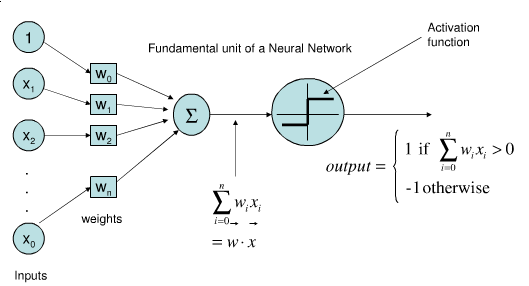
\includegraphics[scale=0.5]{images/perceptron.png}
\end{center}
The model described in the image above is called \textbf{Perceptron}. It first computes the dot-product between the weights $\textbf{w}$ and the input $\textbf{x}$. The result of this computation is usually called $net$
\[net = \sum_{i=0}^{n}w_{i}x_{i}\]
The final output is obtained by applying the \textbf{step function} to the $net$.
\[o = \sigma(net) = sign(net)\]
We will refer to this neuron (and associated learning algorithm) as Perceptron.\newline\newline
Since the hypothesis space of the Perceptron is defined as the hyperplanes in $\mathbb{R}^{n}$, it converges only if the examples in $\mathbb{R}^{n}$ are \textbf{linearly separable}. Otherwise, it will never \textit{find} a hyperplane that separates them.
\subsection{Perceptron: learning algorithm}
Assume to have training examples in $\mathbb{R}^{n}$ that are linearly separable:\newline\newline
Input: Training set $S = \{(\textbf{x}, t), \textbf{x} \in \mathbb{R}^{n+1}, t \in \{-1, +1\}, \eta \geq 0\}$
\begin{enumerate}
    \item Initialize the value of the weights $\textbf{w}$ randomly;
    \item Repeat (N epochs)
    \begin{enumerate}
        \item Select (randomly) one of the training examples $(\textbf{x}, t)$
        \item if $o = sign(\textbf{w} \cdot \textbf{x}) \neq t$ then
        \[\textbf{w} \leftarrow \textbf{w} + \eta(t-o)\textbf{x}\]
    \end{enumerate}
\end{enumerate}
A small value of the learning rate $\eta$ can make the learning process slow but more stable, that is, it prevents sharp changes in the weights vector. If the training set is linearly separable, it can be shown that the Perceptron training algorithm terminates in a finite number of steps.\newline\newline
Let $R$ be the radius of the \textbf{smallest} hyper-sphere centered in the origin enclosing all the instances (how the instances are \textit{spread out}). Let $\gamma$ be the maximal value such that $t_{i}net_{i} = t_{i}(\textbf{w} \cdot \textbf{x}_{i}) \geq \gamma > 0$ (how much the instances are \textit{separated}). Then, it can be shown that the number of steps of the Perceptron algorithm is bounded from above by the quantity $R^{2}/\gamma^{2}$. Basically, bigger \textit{distance} between instances means a smaller number of steps to converge and vice versa.
